%% abtex2-modelo-artigo.tex, v<VERSION> laurocesar
%% Copyright 2012-<COPYRIGHT_YEAR> by abnTeX2 group at http://www.abntex.net.br/ 
%%
%% This work may be distributed and/or modified under the
%% conditions of the LaTeX Project Public License, either version 1.3
%% of this license or (at your option) any later version.
%% The latest version of this license is in
%%   http://www.latex-project.org/lppl.txt
%% and version 1.3 or later is part of all distributions of LaTeX
%% version 2005/12/01 or later.
%%
%% This work has the LPPL maintenance status `maintained'.
%% 
%% The Current Maintainer of this work is the abnTeX2 team, led
%% by Lauro César Araujo. Further information are available on 
%% http://www.abntex.net.br/
%%
%% This work consists of the files abntex2-modelo-artigo.tex and
%% abntex2-modelo-references.bib
%%

% ------------------------------------------------------------------------
% ------------------------------------------------------------------------
% abnTeX2: Modelo de Artigo Acadêmico em conformidade com
% ABNT NBR 6022:2018: Informação e documentação - Artigo em publicação 
% periódica científica - Apresentação
% ------------------------------------------------------------------------
% ------------------------------------------------------------------------


\documentclass[
	% -- opções da classe memoir --
	article,			% indica que é um artigo acadêmico
	11pt,				% tamanho da fonte
	oneside,			% para impressão apenas no recto. Oposto a twoside
	a4paper,			% tamanho do papel. 
	twocolumn,
	% -- opções da classe abntex2 --
	%chapter=TITLE,		% títulos de capítulos convertidos em letras maiúsculas
	%section=TITLE,		% títulos de seções convertidos em letras maiúsculas
	%subsection=TITLE,	% títulos de subseções convertidos em letras maiúsculas
	%subsubsection=TITLE % títulos de subsubseções convertidos em letras maiúsculas
	% -- opções do pacote babel --
	english,			% idioma adicional para hifenização
	brazil,				% o último idioma é o principal do documento
	sumario=tradicional
	]{abntex2}


% ---
% PACOTES
% ---



% ---
% Pacotes fundamentais 
% ---
\usepackage{verbatim}
\usepackage{lmodern}			% Usa a fonte Latin Modern
\usepackage[T1]{fontenc}		% Selecao de codigos de fonte.
\usepackage[utf8]{inputenc}		% Codificacao do documento (conversão automática dos acentos)
\usepackage{indentfirst}		% Indenta o primeiro parágrafo de cada seção.
\usepackage{nomencl} 			% Lista de simbolos
\usepackage{color}				% Controle das cores
\usepackage{graphicx}			% Inclusão de gráficos
\usepackage{microtype} 			% para melhorias de justificação
\usepackage{titlesec}
% ---
		
% ---
% Pacotes adicionais, usados apenas no âmbito do Modelo Canônico do abnteX2
% ---
\usepackage{lipsum}				% para geração de dummy text
% ---
		
% ---
% Pacotes de citações
% ---
\usepackage[brazilian,hyperpageref]{backref}	 % Paginas com as citações na bibl
\usepackage[alf]{abntex2cite}	% Citações padrão ABNT
% ---

% ---
% Configurações do pacote backref
% Usado sem a opção hyperpageref de backref
\renewcommand{\backrefpagesname}{Citado na(s) página(s):~}
% Texto padrão antes do número das páginas
\renewcommand{\backref}{}
% Define os textos da citação
\renewcommand*{\backrefalt}[4]{
	\ifcase #1 %
		Nenhuma citação no texto.%
	\or
		Citado na página #2.%
	\else
		Citado #1 vezes nas páginas #2.%
	\fi}%
% ---


\titleformat{\chapter}     {\normalfont\normalsize\bfseries}{\thechapter}     				 {1em}{}
\titleformat{\section}     {\normalfont\normalsize}{\thechapter.\thesection}     			 {1em}{}
\titleformat{\subsection}  {\normalfont\normalsize}{\thechapter.\thesection.\thesubsection}  {1em}{}
% \renewcommand*{\thesubsection}{\alph{subsection})}

% --- Informações de dados para CAPA e FOLHA DE ROSTO ---
\titulo{Circuito digital CMOS para controle do fator de qualidade de um filtro passa banda-ativo sintonizável}
\tituloestrangeiro{Testing}

\autor{
Alef de Oliveira Santos, Dean Bicudo Karolak, Paulo Márcio Moreira e Silva
}

\local{Brasil}
\data{2018, v<VERSION>}
% ---

% ---
% Configurações de aparência do PDF final

% alterando o aspecto da cor azul
\definecolor{blue}{RGB}{41,5,195}

% informações do PDF
\makeatletter
\hypersetup{
     	%pagebackref=true,
		pdftitle={\@title}, 
		pdfauthor={\@author},
    	pdfsubject={Modelo de artigo científico com abnTeX2},
	    pdfcreator={LaTeX with abnTeX2},
		pdfkeywords={abnt}{latex}{abntex}{abntex2}{atigo científico}, 
		colorlinks=true,       		% false: boxed links; true: colored links
    	linkcolor=blue,          	% color of internal links
    	citecolor=blue,        		% color of links to bibliography
    	filecolor=magenta,      		% color of file links
		urlcolor=blue,
		bookmarksdepth=4
}
\makeatother
% --- 

% ---
% compila o indice
% ---
\makeindex
% ---

% ---
% Altera as margens padrões
% ---
\setlrmarginsandblock{1.5cm}{1.5cm}{*}
\setulmarginsandblock{1.5cm}{2.5cm}{*}
\checkandfixthelayout
% ---

% --- 
% Espaçamentos entre linhas e parágrafos 
% --- 

% O tamanho do parágrafo é dado por:
\setlength{\parindent}{1.3cm}

% Controle do espaçamento entre um parágrafo e outro:
\setlength{\parskip}{0.2cm}  % tente também \onelineskip

% Espaçamento simples
\SingleSpacing


% ----
% Início do documento
% ----
\begin{document}

% Seleciona o idioma do documento (conforme pacotes do babel)
%\selectlanguage{english}
\selectlanguage{brazil}

% Retira espaço extra obsoleto entre as frases.
\frenchspacing 

% ----------------------------------------------------------
% ELEMENTOS PRÉ-TEXTUAIS
% ----------------------------------------------------------

%---
%
% Se desejar escrever o artigo em duas colunas, descomente a linha abaixo
% e a linha com o texto ``FIM DE ARTIGO EM DUAS COLUNAS''.
% \twocolumn[    		% INICIO DE ARTIGO EM DUAS COLUNAS
%
%---

% página de titulo principal (obrigatório)
% \maketitle
% titulo em outro idioma (opcional)

\twocolumn[
	\begin{center}
		% % \begin{minipage}[H]{0.4}
		% % 	\begin{figure*}[]
		% % 		\centering
		% % 		
\includegraphics[H]{./unifeilogo.eps}
				
		% % 	\end{figure*}
			
		% % \end{minipage}
		% \begin{minipage}
			
		% \end{minipage}
		\Large 
		 	Trabalho de conclusão de curso \\
		 	Universidade Federal de Itajubá - \textit{Campus} Theodomiro Carneiro Santiago\\
			Instituto de Ciências Tecnológicas - ICT\\
			\large
			Engenharia de Computação
		
		\normalsize
			
			
			\vspace*{1cm}
			\textbf{\imprimirtitulo}
			\vspace*{1cm}

			Alef de Oliveira Santos${}^*$, Dean Bicudo Karolak${}^*$, Paulo Márcio Moreira e Silva${}^*$

			\vspace*{0.5cm}

			${}^*$\textit{Universidade Federal de Itajubá - Campus Theodomiro Carneiro Santiago \\ Rua Rua Irmã Ivone Drumond, 200 - Distrito Industrial II - 35903-087 \\
			Itabira, Minas Gerais, Brasil} \\

			\vspace*{0.5cm}

			\textit{E-mail}: 
				\href{mailto:alef_santos@unifei.edu.br}{\verb|alef\_santos@unifei.edu.br}, 
				\href{mailto:dean.karolak@unifei.edu.br}{\verb|dean.karolak@unifei.edu.br},
				\href{mailto:paulo.silva@unifei.edu.br }{\verb|paulo.silva@unifei.edu.br } 
		
		
	\end{center}

	\begin{abstract}
		teste
	\end{abstract}


	\begin{resumo}
		teste
	\end{resumo}

	\textbf{Abstract:}\\
	\textbf{Keywords:}\\
	\textbf{Resumo:}\\
	\textbf{Palavras-Chave:}\\
]


% resumo em português
% \begin{resumoumacoluna}
%  Conforme a ABNT NBR 6022:2018, o resumo no idioma do documento é elemento obrigatório. 
%  Constituído de uma sequência de frases concisas e objetivas e não de uma 
%  simples enumeração de tópicos, não ultrapassando 250 palavras, seguido, logo 
%  abaixo, das palavras representativas do conteúdo do trabalho, isto é, 
%  palavras-chave e/ou descritores, conforme a NBR 6028. (\ldots) As 
%  palavras-chave devem figurar logo abaixo do resumo, antecedidas da expressão 
%  Palavras-chave:, separadas entre si por ponto e finalizadas também por ponto.
 
%  \vspace{\onelineskip}
 
%  \noindent
%  \textbf{Palavras-chave}: latex. abntex. editoração de texto.
% \end{resumoumacoluna}


% % resumo em inglês
% \renewcommand{\resumoname}{Abstract}
% \begin{resumoumacoluna}
%  \begin{otherlanguage*}{english}
%    According to ABNT NBR 6022:2018, an abstract in foreign language is optional.

%    \vspace{\onelineskip}
 
%    \noindent
%    \textbf{Keywords}: latex. abntex.
%  \end{otherlanguage*}  
% \end{resumoumacoluna}

% % ]  				% FIM DE ARTIGO EM DUAS COLUNAS
% % ---

% \begin{center}\smaller
% \textbf{Data de submissão e aprovação}: elemento obrigatório. Indicar dia, mês e ano

% \textbf{Identificação e disponibilidade}: elemento opcional. Pode ser indicado 
% o endereço eletrônico, DOI, suportes e outras informações relativas ao acesso.
% \end{center}

% ----------------------------------------------------------
% ELEMENTOS TEXTUAIS
% ----------------------------------------------------------
\textual

% ----------------------------------------------------------
% Introdução
% ----------------------------------------------------------
\chapter{Introdução}

Este documento e seu código-fonte são exemplos de referência de uso da classe
\textsf{abntex2} e do pacote \textsf{abntex2cite}. O documento exemplifica a
elaboração de publicação periódica científica impressa produzida conforme a ABNT
NBR 6022:2018 \emph{Informação e documentação - Artigo em publicação periódica
científica - Apresentação}.

A expressão ``Modelo canônico'' é utilizada para indicar que \abnTeX\ não é
modelo específico de nenhuma universidade ou instituição, mas que implementa tão
somente os requisitos das normas da ABNT. Uma lista completa das normas
observadas pelo \abnTeX\ é apresentada em \citeonline{abntex2classe}.

Sinta-se convidado a participar do projeto \abnTeX! Acesse o site do projeto em
\url{http://www.abntex.net.br/}. Também fique livre para conhecer,
estudar, alterar e redistribuir o trabalho do \abnTeX, desde que os arquivos
modificados tenham seus nomes alterados e que os créditos sejam dados aos
autores originais, nos termos da ``The \LaTeX\ Project Public
License''\footnote{\url{http://www.latex-project.org/lppl.txt}}.

Encorajamos que sejam realizadas customizações específicas deste documento.
Porém, recomendamos que ao invés de se alterar diretamente os arquivos do
\abnTeX, distribua-se arquivos com as respectivas customizações. Isso permite
que futuras versões do \abnTeX~não se tornem automaticamente incompatíveis com
as customizações promovidas. Consulte \citeonline{abntex2-wiki-como-customizar}
para mais informações.

Este exemplo deve ser utilizado como complemento do manual da classe
\textsf{abntex2} \cite{abntex2classe}, dos manuais do pacote
\textsf{abntex2cite} \cite{abntex2cite,abntex2cite-alf} e do manual da classe
\textsf{memoir} \cite{memoir}. Consulte o \citeonline{abntex2modelo} para obter
exemplos e informações adicionais de uso de \abnTeX\ e de \LaTeX.


\chapter{Introdução}

% o que é o quê e por quê ele é importante?
% como medir o Q
% [ENFASE] como controlar o Q 
% 

Este trabalho trata de um sistema eletrônico que recebe e controla o fator de qualidade ($Q$) de um circuito eletrônico ressonante. O circuito proposto utiliza-se de técnicas de computação numérica para controlar o fator de qualidade através de uma corrente de referência injetada no sistema ressonante. Neste trabalho serão realizados circuitos digitais periféricos para a determinação do valor de $Q$ medido de um filtro passa banda ativo, bem como, um circuito digital para controle e aproximação do $Q$ desejado. Em relação ao controle e aproximação de Q, serão comparados os métodos numéricos da Bisseção, Secantes e Secantes com seleção de intervalo implementados. O sistema digital é projetado e implementado em Verilog tendo em mente a posterior fabricação em silício. Para efeitos de estudo e desenvolvimento, este projeto em ASIC utiliza uma tecnologia GPDK de 45nm.

% Neste trabalho serão realizados circuitos digitais periféricos para a determinação do valor de Q medido de um filtro passa banda ativo, bem como, um circuito digital para controle e aproximação do Q desejado. Em relação ao controle e aproximação de Q, serão comparados...

\section{Contexto e justificativa}

A caracterização fator de qualidade ($Q$) é um ponto de partida para projetos de circuitos integrados de rádio-frequência de alto desempenho \cite{what-is-q-takashi}. Ele está relacionado com a largura de banda de um filtro passa-banda e, por vezes, os projetistas de filtros necessitam de uma largura de banda estreita (isto é, alto $Q$) e em outras, uma banda maior (baixo $Q$) como ilustra a \autoref{f-banda-q}:

\begin{figure}[H]
    \centering
    \caption{$Q$ \textit{versus} largura de banda}
    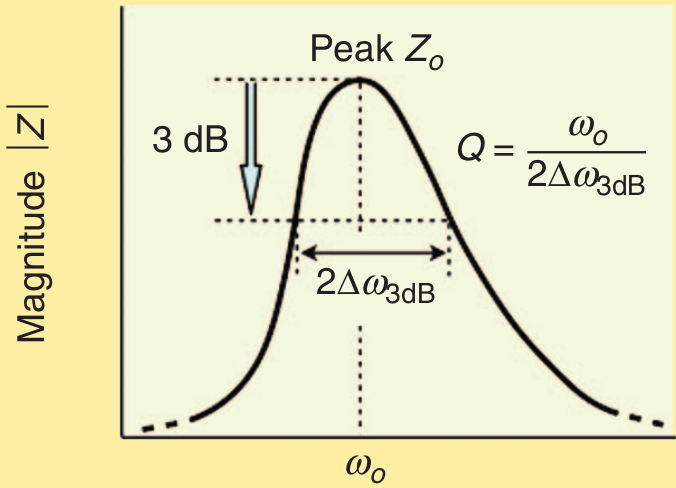
\includegraphics[width=.5\textwidth]{fig/q-band.png}
    \legend{Fonte: \cite{what-is-q-takashi}}
    \label{f-banda-q}
\end{figure}

% Da teoria de sistemas de controles dinâmicos, mudar a resposta em frequência do projeto de filtros,

% No trabalho de \autoref{z-matching}

Ainda de acordo com \citeauthor{what-is-q-takashi}, o fator $Q$ também está relacionado com o teorema da máxima transferência de potência em circuitos de RF. Para entregar o máximo de potência de uma fonte para uma carga através de uma rede, um circuito de casamento de impedâncias é usado para alcançar a maior transferência de potência. A \autoref{f-eff-q} ilustra como o $Q$ interfere na eficiência de um circuito:


\begin{figure}[H]
    \centering
    \caption{$Q$ \textit{versus} eficiência}
    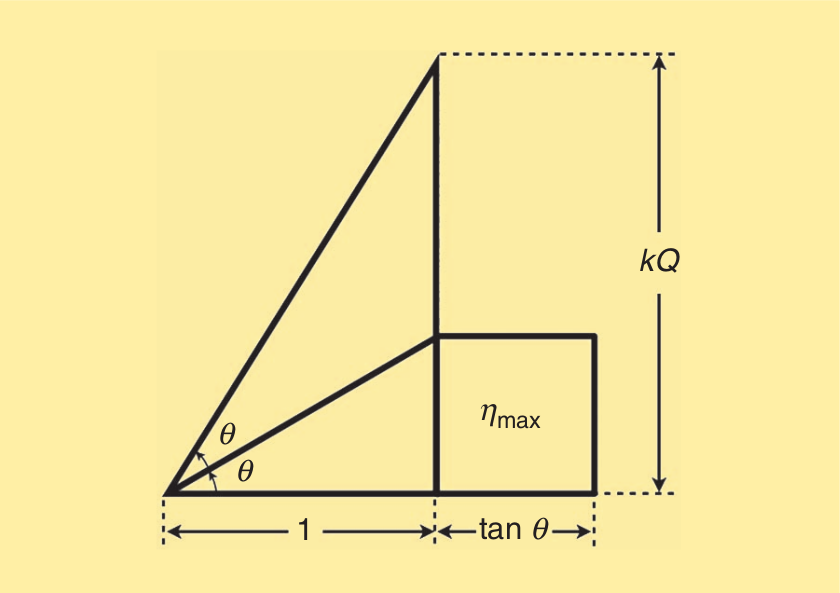
\includegraphics[width=.5\textwidth]{fig/q-eff.png}
    \legend{Fonte: \cite{what-is-q-takashi}}
    \label{f-eff-q}
\end{figure}


Num circuito com uma carga estática, basta calcular um $Q$ que realize o casamento de impedâncias para a maior transferência de potência. Num circuito onde a carga é variável, um $Q$ fixo não fornece o casamento de impedâncias necessário para a máxima transferência de potência em todos os cenários de carregamento, assim reduzindo a eficiência do circuito. 

De fato \citeauthor{z-match-q} retomam em seu trabalho as proposições de \citeauthor{what-is-q-takashi} e projetam uma rede de casamentos de impedância baseada no fator de qualidade, onde o mesmo é ajustado a fim de casar impedâncias de rede com uma carga variável. \citeauthor{z-match-q-2} realiza um trabalho com a mesma ideia de controlar o $Q$ usando outras técnicas para selecionar o valor ótimo.


% Em sistemas sensores microeletromecânicos (MeMS) o fator de qualidade está atrelado à resolução e à estabilidade em frequência. Um baixo $Q$ resulta em baixa resolução e alta estabilidade em  altas frequências, enquanto um $Q$ alto é o inverso dessas características  \cite{mems-two-inductors}. 

% No trabalho de \citeauthor{mems-two-inductors} foram utilizados dois indutores, sendo um com baixo fator de qualidade e outro com alto, para combiná-los em série e obter um $Q$ intermediário com sensibilidade e estabilidade em frequência suficientes para a aplicação proposta. Sob essa perspectiva, o trabalho aqui desenvolvido seria um adicional relevante pois seria necessário projetar no trabalho de  \citeauthor{mems-two-inductors} apenas um indutor com alto fator de qualidade e controlar o $Q$ da mesma forma proposta neste trabalho. Isso se torna particularmente ainda mais relevante uma vez que o oscilador usado no trabalho de \citeauthor{mems-two-inductors} é similar ao oscilador LC de par cruzado usado neste trabalho, vide \autoref{f-osciladores}.

% % \begin{figure}[H]
% %     \centering
% %     \caption{\textcolor{red}{Comparação entre osciladores usados}}
% %     \begin{subfigure}[H]{.49\textwidth}
% %         \centering
% %         \caption{Oscilador usado neste trabalho}
% %         % 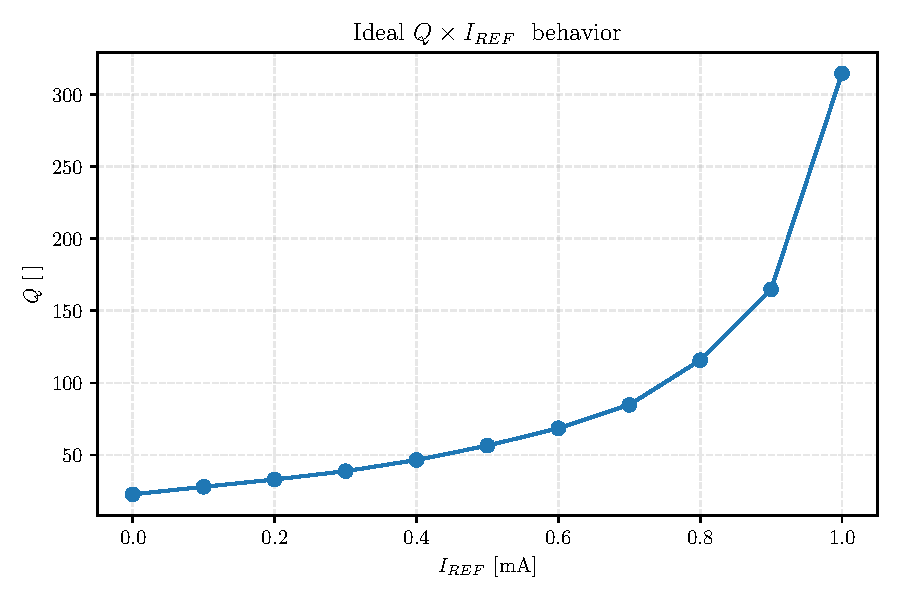
\includegraphics{fig/q-no-drop.pdf}
% %         \legend{Fonte: Adaptado de \cite{tese-pmms}}
% %         % \label{}
% %     \end{subfigure}
% %     \hfil
% %     \begin{subfigure}[H]{.49\textwidth}
% %         \centering
% %         \caption{Oscilador do trabalho de \citeauthor{mems-two-inductors}}
% %         % 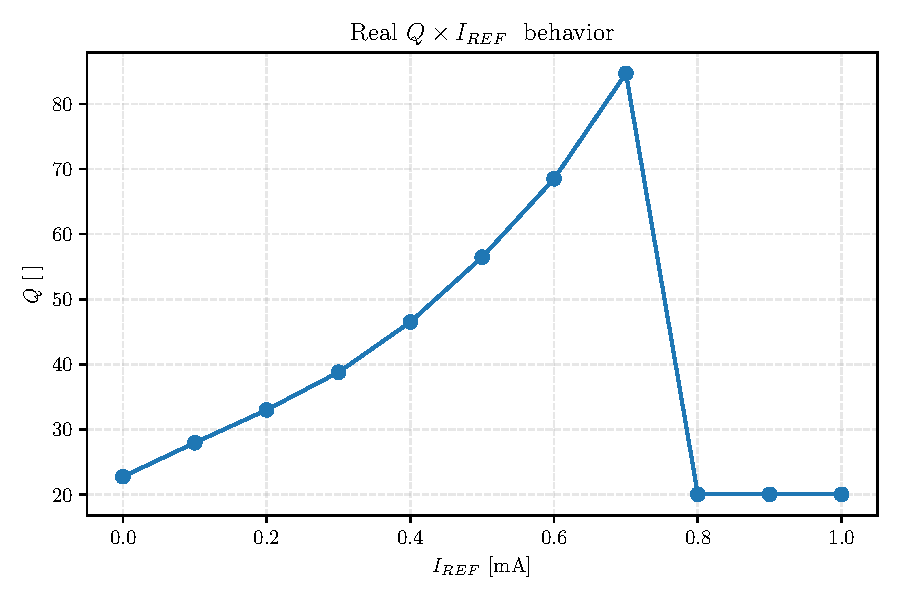
\includegraphics{fig/q-with-drop.pdf}
% %         \legend{Fonte: \cite{mems-two-inductors}}
% %         % \label{}
% %     \end{subfigure}
% %     \hfil
% %     \label{f-osciladores}
% % \end{figure}

% Vistas as similaridades dos osciladores usados, adaptar o circuito de \citeauthor{mems-two-inductors} para o trabalho em questão, usando um único indutor integrado de alto fator de qualidade
% pode ser uma opção viável. De fato projetar um único indutor de alto $Q$ não é tarefa trivial mas a indústria de RF têm avançado e é possível ver indutores com fatores elevados de qualidade, assim como desenvolvidos nos trabalhos de \citeonline{high-q-1} e \citeonline{high-q-2}.


Desta forma, fica evidente a necessidade de controlar o $Q$ de um circuito eletrônico, tanto no contexto deste trabalho quanto em outros trabalhos com pouca similaridade, mas com a mesma necessidade de $Q$ controlável/variável. 


Em relação às diferentes implementações de circuitos eletrônicos para controle do $Q$, pode-se distingui-los em dois grupos, os circuitos analógicos e os digitais. Os circuitos analógicos têm a vantagem de ser mais simples, mais rápidos, como apresentado em \cite{z-match-q-2}. Entretanto, eles não apresentam a mesma versatilidade e configurabilidade proposta por um sistema digital. Já os circuitos digitais, além de mais versáteis, apresentam uma implementação física mais simples com o uso de \textit{standard-cells} para a construção de \textit{layouts}, sendo inclusive, altamente assistidas por ferramentas de EDA pela característica programática. Em conjunto com a maior versatilidade, o circuito digital poderia ser estendido em aplicações onde o controle do $Q$ deve ter alta precisão, uma vez que o circuito digital pode ser replicado com maior confiabilidade, portabilidade e reprodutibilidade. \\



% \begin{itemize}
%     \item \textit{Layout}: O processo de layout digital utilizando-se de \textit{standard cells} é mais rápido e simples de se fazer comparado ao \textit{layout} analógico \cite{the-art-of-layout}
% \end{itemize}


Dessa forma, julga-se pertinente projetar este circuito eletrônico digital capaz de controlar o $Q$, para que seja possível obter circuitos mais versáteis e com aplicações mais amplas com menor complexidade em projeto analógico, além de promover inovação no desenvolvimento de circuitos para computação numérica.





% \section{Trabalhos similares}



\chapter{Objetivos}\label{ch-obj}

Os objetivos principais deste trabalho para o TCC1 são, principalmente o fluxo de front-end, compreendido por:

\begin{enumerate}
    \item Projetar a arquitetura capaz de controlar o fator de qualidade do circuito;
    % \item Adaptar métodos numéricos e prototipá-los em alto nível
    \item Codificar os blocos do sistema projetado em Verilog;
    \item Comparar o desempenho dos métodos de controle prototipados \textit{standalone};
    \item Validar a funcionalidade blocos projetados através de \textit{testbenches} em Verilog/SystemVerilog.
\end{enumerate}


Após finalizado o fluxo de front-end, seleciona-se o método de convergência com melhor desempenho com relação à todo o sistema e inicia-se o processo de verificação do sistema completo seguido do fluxo de back-end no TCC2, compreendido por:

\begin{enumerate}
    \item Integrar e coordenar a operação dos blocos como um sistema completo;
    \item Realizar a síntese lógica em RTL;
    \item Simular o circuito sintetizado em RTL e checar a equivalência lógica;
    \item Realizar etapas de posicionamento e roteamento;
    \item Analisar o consumo;
    \item Analisar desempenho do sistema por temporização estática (STA);
    \item Construir layout.
\end{enumerate}


% ----------------------------------------------------------
% ELEMENTOS PÓS-TEXTUAIS
% ----------------------------------------------------------
\postextual

% ----------------------------------------------------------
% Referências bibliográficas
% ----------------------------------------------------------
\bibliography{ref}

\end{document}
